\documentclass[12pt,article,oldfontcommands]{memoir}

\setlrmarginsandblock{1.2in}{1.2in}{*}
\setulmarginsandblock{1.0in}{1.0in}{*}
\checkandfixthelayout
\setlength{\parindent}{0pt}
\setlength{\parskip}{6pt}

\settocdepth{subsection}
\setcounter{secnumdepth}{0}
\setcounter{maxsecnumdepth}{0}
% \setsecheadstyle{\normalfont\large\sffamily\bfseries\MakeUppercase}
% \setsubsecheadstyle{\normalfont\sffamily\bfseries}
% \renewcommand{\abstractnamefont}{\normalfont\sffamily\MakeUppercase}
% \renewcommand{\abstracttextfont}{\normalfont\sffamily}
\renewcommand{\absnamepos}{center}
\abstractrunin
\captionnamefont{\small}
\captiontitlefont{\small}

\pretitle{\raggedright\LARGE\bfseries}
\posttitle{\par \vskip 0.5 em}
% \preauthor{\lineskip 0.5 em \begin{tabular}[t]{l} \large}
% \postauthor{\end{tabular} \par}
\preauthor{\normalfont \par \vskip 2 em \noindent}
\postauthor{\normalfont \par \vskip 2 em}
\predate{}
\postdate{}
% \setsecheadstyle{\large\sfseries}
% \setbeforesecskip{\baselineskip}
% \setaftersecskip{\baselineskip}
\firmlists

\usepackage{amssymb,amsfonts,amsmath}
\usepackage[minionint,textlf,mathlf]{MinionPro}
\usepackage[scaled=0.90]{helvet}
\usepackage[scaled=0.90]{inconsolata}
\usepackage[]{graphicx}
\usepackage[usenames,dvipsnames]{xcolor}
\usepackage{color}
\usepackage{hyperref}
\usepackage{nameref}

\usepackage[round,numbers,sort&compress]{natbib} 
\bibliographystyle{biophysj}
\renewcommand{\bibnumfmt}[1]{#1.}
\newcommand{\indt}{\qquad}

%% OPTIONAL MACRO DEFINITIONS

% symbols
\renewcommand{\L}{\ensuremath{L}}
\newcommand{\Lem}{\ensuremath{L^{\rm em}}}
\newcommand{\Lvb}{\ensuremath{L^{\rm vb}}}
\newcommand{\Leb}{\ensuremath{L^{\rm eb}}}
\newcommand{\Eo}{\ensuremath{\mathcal{E}^{\rm occ}}}
\newcommand{\Er}{\ensuremath{\mathcal{E}^{\rm rate}}}
\newcommand{\Keff}{\ensuremath{K^{\rm eff}}}
\newcommand{\pd}{\partial}
\newcommand{\dg}{\dagger}
\newcommand{\Dkl}{\ensuremath{D_{\rm KL}}}
\newcommand{\T}{\ensuremath{\mathcal{T}}}

% math notation
\newcommand{\argmax}{\operatornamewithlimits{argmax}}
\newcommand{\argmin}{\operatornamewithlimits{argmin}}
\newcommand{\pdff}[2]{\frac{\partial #1}{\partial #2}}
\newcommand{\fdff}[2]{\frac{\delta #1}{\delta #2}}
\newcommand{\ifrac}[2]{#1 \:/\: #2}
\newcommand{\abs}[1]{\left\vert #1 \right\vert}
\newcommand{\ten}[1]{\underline{\underline{#1}}}
\newcommand{\p}[2]{\ensuremath{p(#1 \:|\: #2)}}
\newcommand{\ps}[2]{\ensuremath{p^*(#1 \:|\: #2)}}
\newcommand{\q}[2]{\ensuremath{q(#1 \:|\: #2)}}
\renewcommand{\d}[1]{\ensuremath{\!\!d#1 \:}}

% condensed +/-
\newcommand{\mm}{\ensuremath{\!-\!}}
\newcommand{\pp}{\ensuremath{\!+\!}}
\newcommand{\ee}{\ensuremath{\!=\!}}

% comments
\newcommand{\jwm}[1]{\textcolor{Magenta}{#1}}
\newcommand{\rlg}[1]{\textcolor{Orange}{#1}}
% \newcommand{\jwm}[1]{#1}
% \newcommand{\rlg}[1]{#1}
% \newcommand{\fw}[1]{#1}
% \newcommand{\wei}[1]{#1}
\newcommand{\com}[1]{[\emph{#1}]}

% shortcuts for priors
\newcommand{\pmu}{{m_{0}}}
\newcommand{\pbeta}{{\beta_{0}}}
\newcommand{\pa}{{a_{0}}}
\newcommand{\pb}{{b_{0}}}
\newcommand{\pnu}{{\nu_{0}}}
\newcommand{\pW}{{W_{0}}}
\newcommand{\ppi}{{\rho_{0}}}
\newcommand{\pA}{{\alpha_{0}}}

% shortcuts for posteriors
\newcommand{\qmu}{m}
\newcommand{\qbeta}{\beta}
\newcommand{\qa}{a}
\newcommand{\qb}{b}
\newcommand{\qnu}{\nu}
\newcommand{\qW}{W}
\newcommand{\qpi}{\rho}
\newcommand{\qA}{\alpha}


\begin{document}
\section*{ebFRET User Guide}
\subsubsection*{Release 1.1, May 2014}

\indt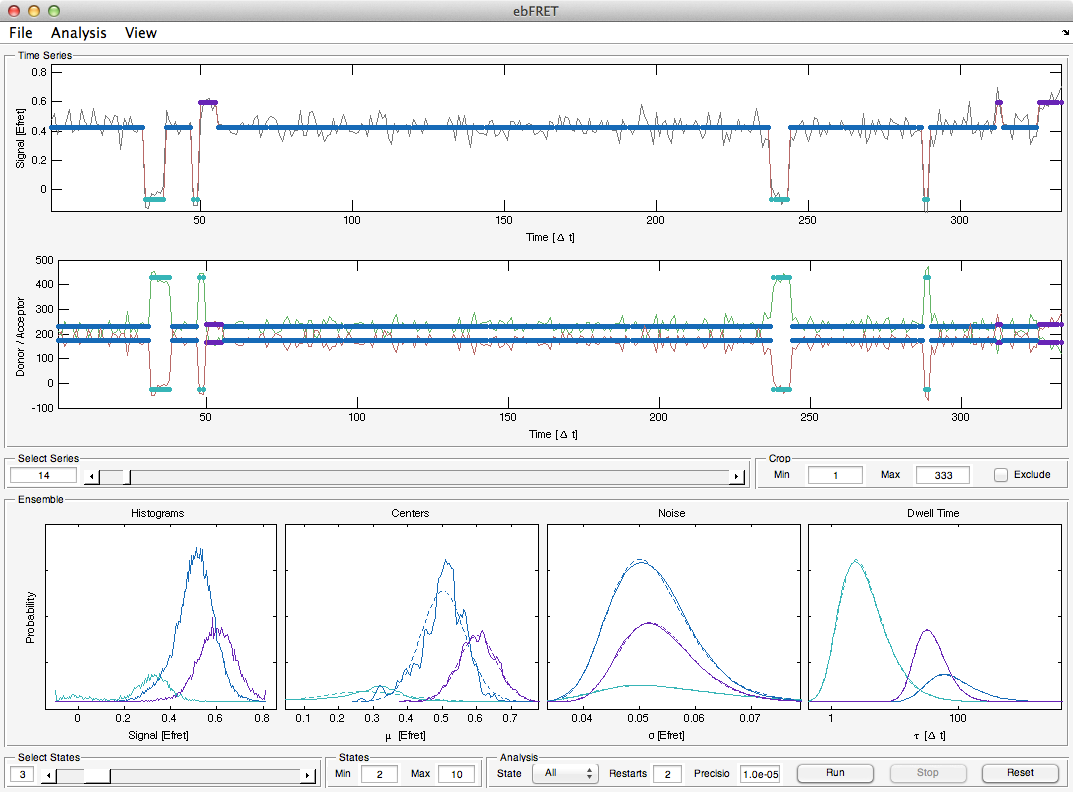
\includegraphics[width=5in]{images/ebfret_mainwindow}

\tableofcontents*



\section{Getting Started}
\label{Getting Started}

\subsection{Quick Usage}

\begin{itemize}
\item[1.] Download the latest version of ebFRET from

\indt\url{https://github.com/ebfret/ebfret-gui/archive/master.zip}

\item[2.] Unzip the folder to some location, e.g. 
\begin{verbatim}
    C:\path\to\ebFRET
\end{verbatim}

\item[3.] Start up Matlab and add the ebFRET to the path by typing
\begin{verbatim}
    addpath(genpath(C:\path\to\ebFRET))
\end{verbatim}
\item[4.] Open the GUI by typing 
\begin{verbatim}
    ebFRET()
\end{verbatim}

\item[5.] Load an example dataset by clicking \texttt{File} $\to$ \texttt{Load} and select the file 
\begin{verbatim}
    C:\path\to\ebFRET\datasets\simulated-K04-N350-raw-unstacked.dat
\end{verbatim}

\item[6.] Click \texttt{Run} to start analysis

\end{itemize}

\subsection{System Requirements}

\subsubsection{Operating System} 

The ebFRET software suite should in princle run on all operating systems supported by Matlab (i.e. Windows, OS X and Linux). Development and testing was done with Matlab 2013a on OS X (Mountain Lion) and Windows 7.

\subsubsection{Matlab Version} 

We recommend using a Matlab version $\ge$ 2012a. The GUI has been verified to work with Matlab versions as early as 2010b, but may exhibit performance issues related to the slower implementations of object-oriented programming methods in versions prior to 2012a.

\subsubsection{Memory Requirements}

Memory requirements vary depending on the size of the dataset, the number of states, and the number of CPUs used. Typically, memory usage of a single instance should be less than 1 GB for moderately large datasets containing order $10^5$ total datapoints in all time series. 

\subsubsection{MEX Files}

In order to achieve higher performance, some parts of the ebFRET code are written as MEX files in C. These functions may need to be compiled after installation. The ebFRET GUI attempts to do so automatically as needed, but this process will fail if the prerequisite compilers are not installed. In this event ebFRET will revert to using (slower) functions written in Matlab and print a warning message. For more information, see the \emph{\nameref{sec:advanced}} section.

\subsection{Installation}

\subsubsection{Obtaining the Source Code}

The latest version of the source for  the ebFRET package may be obtained by visiting 

\indt\url{https://ebfret.github.io}

A zip file containing the sources can be found at 

\indt\url{https://github.com/ebfret/ebfret-gui/archive/master.zip}

Alternatively the source may be obtained using \texttt{git} 
\begin{verbatim}
    git clone git@github.com/ebfret/ebfret-gui.git
\end{verbatim}

\subsubsection{Adding the ebFRET Source to the Matlab path}

Once the ebFRET source file has been downloaded (and unzipped), it must be added to the Matlab path. This can be via 

\indt\texttt{Environment} $\to$ \texttt{"Set Path"} $\to$ \texttt{"Add with Sub-folders"} (Matlab $\ge 2013a$)

% \indt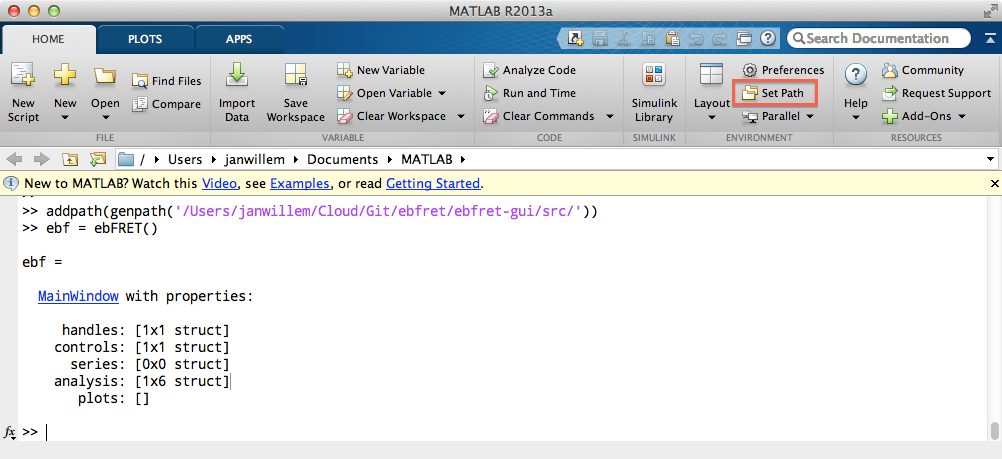
\includegraphics[width=5.5in]{images/matlab_2013a_set_path}

\indt\texttt{File} $\to$ \texttt{"Set Path"} $\to$ \texttt{"Add with Sub-folders"} (Matlab $< 2013a$)

% \indt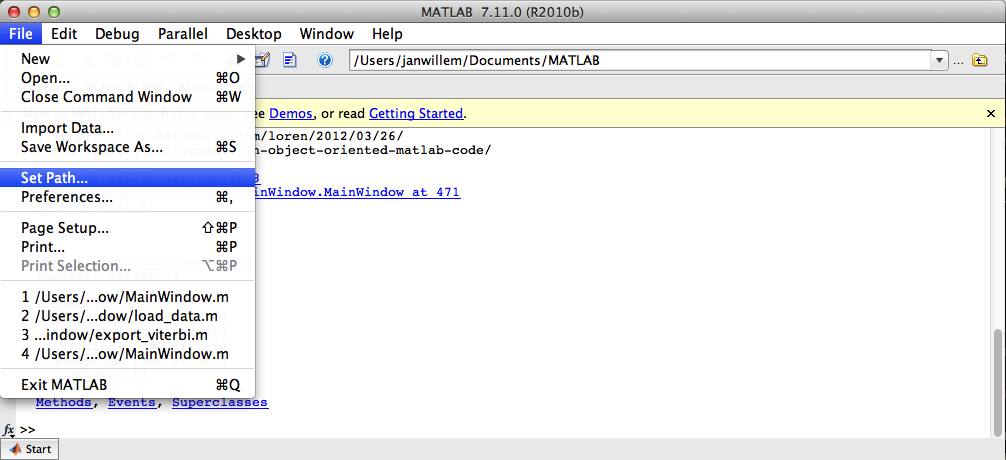
\includegraphics[width=5.5in]{images/matlab_2010b_set_path}

 Once the folder is added to the path, \texttt{Save} may be use to ensure the new path is retained in future Matlab sessions. 

\indt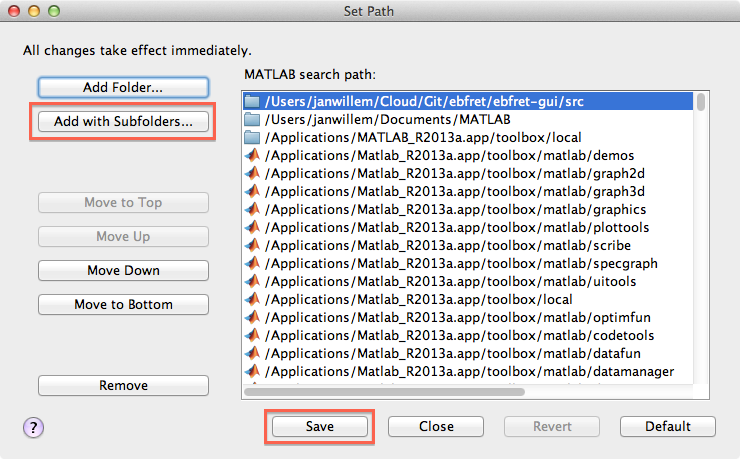
\includegraphics[width=4in]{images/matlab_2013a_set_path_dialog}


 Alternatively, the folder containing the ebFRET source 
(e.g. \verb|C:\path\to\ebFRET|) may be added by to the path via the command
\begin{verbatim}
    addpath(genpath(C:\path\to\ebFRET))
\end{verbatim}

\subsubsection{Starting the GUI}

To open a new instance of the ebFRET GUI, simply type
\begin{verbatim}
    ebf = ebFRET()
\end{verbatim}
The returned object handle \texttt{ebf} is a matlab object that provides access to the entire GUI state. In particular, the loaded time series may be accessed via \texttt{ebf.series}, and the analysis results can be found in \texttt{ebf.analysis}. Accessing these values directly is not necessary in normal usage, but can be helpful if custom pre-processing or post-processing is needed. See the \emph{\nameref{sec:advanced}} section for futher information.

\section{Loading Data}

Data can be loaded into the gui via the \texttt{File} $\to$ \texttt{Load}~ menu item. ebFRET currently supports loading data from a number of different formats.

\subsection{File Formats}

\begin{itemize}
\item[\textbf{1.}] \textbf{ebFRET saved session (.mat)}

Loading from this format restores an ebFRET session saved via \texttt{File} $\to$ \texttt{Save}. This file contains all data necessary to continue analysis from the point at which the file was saved. 

\textbf{\item[2.] Raw donor-acceptor time series (.dat)}

This loads a number of FRET time series from an ASCII file, which may be stored in two ways, which we call `stacked' and `unstacked'. Example data stored in both formats can be found in the \texttt{examples} sub-directory of the ebFRET folder. 

\begin{itemize}
\item[\emph{a.}] \emph{Stacked}

The stacked format is useful for storing time series with variable length. Let's assume we have $N$ time series, with length $T(n)$, and intensities $D(n,t)$ and $A(n,t)$ for the donor and acceptor respectively. Each row in a stacked table now contains 3 values 
\begin{verbatim}
     label(1)    D(1,1)       A(1,1)
     label(1)    D(1,2)       A(1,2)
     ... 
     label(1)    D(1,T(1))    A(1,T(1))
     ...
     ...
     label(N)    D(N,T(N))    A(N,T(N))  
\end{verbatim}
Where \texttt{label(n)} is a numeric unique id for each time series.

\emph{\item[b.] Unstacked}

The unstacked format stores $N$ times series of identical length $T$ in $T \times 2 D$ matrix formatted as 
\begin{verbatim}
     label(1)  label(1)  ...    label(N)  label(N)
     D(1,1)    A(1,1)    ...    D(N,1)    A(N,1)
     D(1,2)    A(1,2)    ...    D(N,2)    A(N,2)
     ...       ...       ...    ...       ...
     D(1,T)    A(1,T)    ...    D(N,T)    A(N,T)
\end{verbatim}

\end{itemize}

\textbf{\item[3.] SFTracer donor-acceptor time series (.tsv)}

This format is used by the SFTracer pre-processing suite for FRET time series, that is currently in preparation for release at the Gonzalez lab at Columbia. This data is stored as tab-separated values (TSV). The first two lines of each file contain meta-information and column headers respectively. The remaining lines store multi-color FRET data as
\begin{verbatim}
    n c area(n) T(n) I0(n,c) I(n,c,1) I(n,c,2) ... I(n,c,T(n))
\end{verbatim}
Here \texttt{c} is the index of the color channel. The GUI assumes \texttt{c==0} for the donor signal and \texttt{c==1} for the acceptor signal. \texttt{T(n)} is the number of time points in time series \texttt{n}, and \texttt{I0(n,c)} is the background intensity of channel \texttt{c} for this time series. \texttt{area(n)} holds the surface area of the spot in the source image, which is currently ignored by ebFRET. 

\textbf{\item[4.] Single-molecule Dataset (.json, .json.gz, .mat)}

The single-molecule dataset (SMD) format may be used to import data exported by other smFRET analysis packages, such as SMART\footnote{\url{https://simtk.org/home/smart}}. 
A SMD file can be read from JSON (\texttt{.json}), gzipped JSON (\texttt{.json.gz}) and Matlab (\texttt{.mat}) formats, and can hold both raw (unanalyzed) data and unanalyzed results. 
Currently only raw time series can be read from SMD files. 
We loading SMD, the user may specified whether the stored time series contain \texttt{Donor-Acceptor} or \texttt{FRET} data. 
For each choice, the user must then select the SMD column names that contain the donor, acceptor, or FRET signals respectively. 

\end{itemize}


\subsection{Loading Data from Multiple Files}

When loading data from Raw or SFTracer formats, it is possible to select multiple files to load several datasets at once. Data can also be added in increments. The GUI will then prompt to either to either retain or replace the existing data. 

\subsection{Grouping Files}

The loading mechanism can implicitly be used to create `groups' of files. For example, if one wishes to obtain separate parameter estimates for 3 sets of experiments, once can load each group separately by clicking \texttt{File} $\to$ \texttt{Load}. When data is loaded in this manner, the \texttt{File} $\to$ \texttt{Export} $\to$ \texttt{"Analysis Summary"} function (see \emph{\nameref{sec:save-export}}) will automatically calculate summary statistics separately for each group. If more sophisticatd grouping criteria are needed, these must be implemented by hand. See the \emph{\nameref{sec:advanced}} section for further information.

\section{Performing Analysis}

\subsection{Exploring the Data}

Once data has been loaded, the main window will display time series plots of the $E_{\rm FRET}$ ratio, as well as the donor and acceptor intensities (shown in green and red respectively).

\indt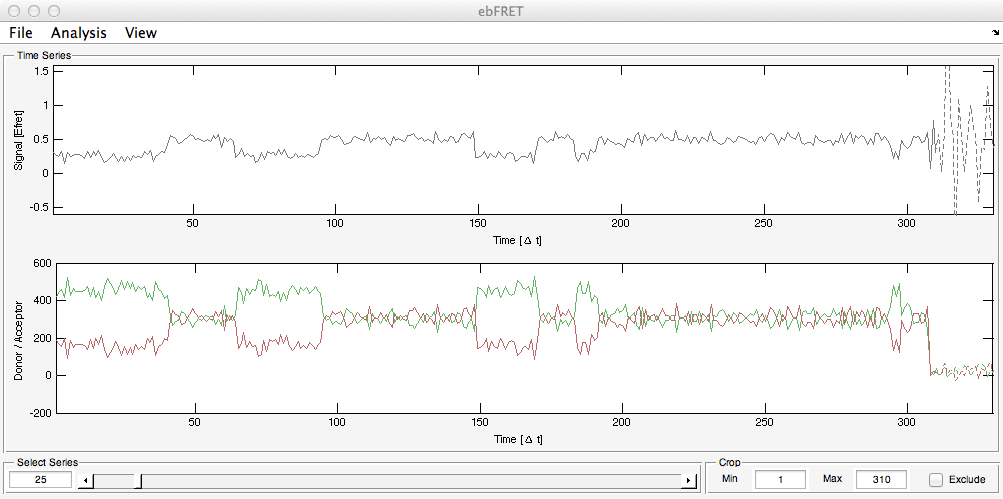
\includegraphics[width=5.5in]{images/trace_view}

The slider in the \texttt{Series} box underneath the plots may be used to view different time series in a dataset, and the edit box beside it may be used to select a specific series.

\subsection{Pre-processing the Data}

\subsubsection{Photobleaching Detection}

\indt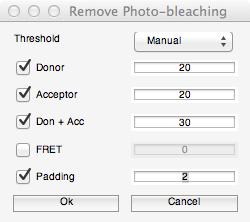
\includegraphics[width=2in]{images/remove_photobleaching_dialog}

A common pre-processing task when working with FRET time series is cropping the time series to the point where either the donor or acceptor fluorophore photobleaches. ebFRET can do so according to several criteria using the dialog accessed via \texttt{Analysis} $\to$ \texttt{"Remove Photobleaching"} 

\begin{itemize}
\item[\textbf{1.}] \textbf{Manual}

In this mode the time series is truncated when a selected value falls below the specified level. It is possible to select multiple criteria, in which case the time series is truncated at the first point that satisfies one of the selected criteria. It is also possible to use a \texttt{Padding} to crop extra time points from the end of the series.

\item[\textbf{2.}] \textbf{Automatic}

In this mode, photobleaching is detected in a fully automated manner, by looking for jumps in the signal starting from the end of the time series. 
\end{itemize}

\subsubsection{Clipping of Outlier Points}

\indt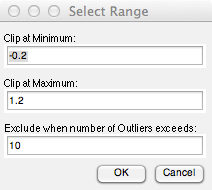
\includegraphics[width=1.8in]{images/clip_outliers_dialog}

Time series in a dataset may exhibit $E_{\rm FRET}$ values that are either $< 0$  or $> 1$. Note that such values can only occur when the acceptor or donor intesities falls below 0, which is by definition an unphysical occurence that typically occurs when the background intensity cannot be determined accurately.

A small number of such outlier points can often significantly skew analyis outcomes. Because of this, it is generally a good idea to either clip outlier points $\ll 0$ and $\gg 0$ to more sanitized values, or exclude time series that exhibit many outlier points from the analysis entirely.
This can be done by adjusting the minimum and maximum thresholds, as well as the maximum number of outliers.

\subsubsection{Manual Correction}

Both photobleaching removal and detection of outliers are non-desctructive operations. What this means is that all the data is retained in its original form, and simply pre-processed as needed when analysis if performed. Both operations can safely be run multiple times to find the best settings, without losing more and more data. 

In addition there are \texttt{Crop} controls that can be used to correct the time interval that is used for analysis, as well as an \texttt{Exclude} button that can be used to entirely remove time series from analysis, or include a previously excluded time series once more.

\subsection{Initializing the Priors}

\subsubsection{Automatic Initialization}

In ebFRET multiple time series are analyzed to determine the `range' of parameter values that best describes an ensemble of parameters. This range of values is described by a probability distribution known a the prior, and the goal when running analysis in ebFRET is to learn this prior from the data. In order to do so, the algorithm must be provided with an intial guess.

When the data is loaded, ebFRET makes an automatic guess for the initial values of the priors. In most case this guess will suffice. However, if there are outliers in the data, the algorithm for generating this initial guess may be a poor fit for the data. For this reason, the ebFRET GUI prompts the user to re-initialize the priors after photobleaching and outlier removal. In most cases the automatically determined result after post-processing should suffice.

\indt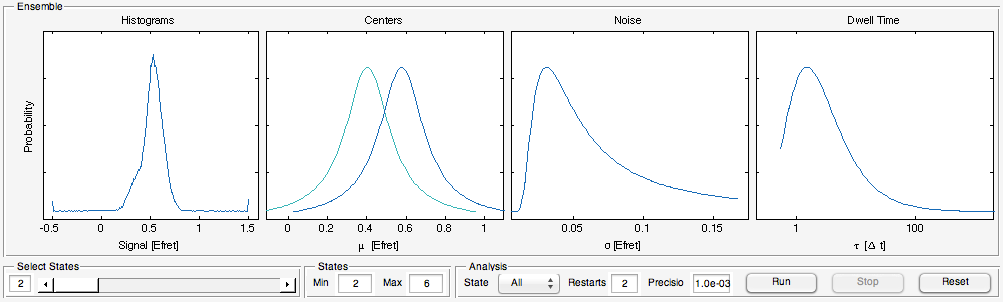
\includegraphics[width=5.5in]{images/ensemble_view}

After initialization, the \texttt{Ensemble} panel shows the distribution of measurement values and parameters. The fist panel shows a simple histogram of measurement values, the second the distribution for state means, which should show a spread of values similar to the measurement histogram. The distributions on state noise levels and dwell times, shown in the 3rd and 4th panels respectively, are by default initialized with identical values.

\subsubsection{Manual Adjustment}

If more precise control is needed, the priors may be adjusted manually using the dialog located under \texttt{Analysis} $\to$ \texttt{"Set Priors"} 

\indt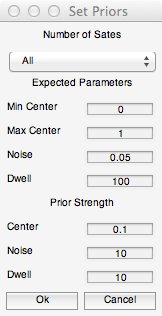
\includegraphics[width=1.2in]{images/set_priors_dialog}

The \texttt{Min Center} and \texttt{Max Center} parameters control the mean $E_{\rm FRET}$ values assumed for each state, which are spaced evenly between the extrema. The \texttt{Noise} parameter controls the expected emission noise around each state, whereas the \texttt{Dwell} parameter contol how many time points are typically spent in one state, before a transition to a different state occurs.

In addition to the expected parameter values, it is also possible to specify a \texttt{Prior Strength} in terms of a number of equivalent observations. If this number is lowered, the prior distributions become more broadly peaked, and describe a larger range of allowable parameter values. When this number is increased, the distribution becomes more tightly peaked, and a smaller range of parameter values is considered.

From experience we find that the initial guess for the prior generally should not strongly affect analysis outcomes. However, the \texttt{Center Strength} parameter can affect performance of the algorithm to some extent. If the \texttt{Strength} parameter is increased, the algorithm will be more likely to populate larger numbers of states. In this case the lower bound evidence must be used to decide among analysis results with different numbers of states. Setting the strength parameter to lower values will make the algorithm more likely to leave superfluous states unpopulated. This should result in consistent analysis outcomes as more states are considered, with correspondingly similar lower bound evidence values. We generally recommend setting the \texttt{Center Strength} parameter as low as possible, while making sure that no obvious features in the data are missed by the analysis.

Finally, priors may also be set directly from command window by manipulating values stored in \texttt{ebf.analysis.prior}. See the \emph{\nameref{sec:advanced}} section for further details.

\subsection{Running Analysis}

Once data has been loaded, pre-processed, and the priors have been intialized, analysis can be started by pressing the \texttt{Run} button.

The ebFRET algorithm performs analysis by repeatedly executing two steps

\begin{itemize}
\item[1.] Use variational Bayes (VB) estimation (i.e. the same method as vbFRET) to learn HMM parameters for each time series.
\item[2.] Use empirical Bayes (EB) estimation to adjust the prior distributions to match the posterior distributions learned for individual time series.
\end{itemize}

The settings that control how analysis is performed by the ebFRET GUI are
\begin{itemize}
\item[\emph{1.}] \emph{States $\to$ Min, Max}

These parameters control the smallest and largest number of states considered. 

\item[\emph{2.}] \emph{Analysis $\to$ State $\to$ All/Current}

When analysis is performed, it is possible to either run analysis only for the \texttt{Current} number of states, shown in the \texttt{Ensemble} view, or for all numbers of state, starting from the minimum. 

\item[\emph{3.}] \emph{Analysis $\to$ Restarts}

This parameter controls the number of re-initializations used each time variational Bayes estimation is performed on an individual time series. If set to 0, VB estimation is performed only once, starting from the final parameters of the previous iteration. If set to 1, an additional `uninformative' restart is performed. If set to values $>$1, further restarts are performed with random initializations.

Using more restarts makes the EB algorithm more likely to converge towards the correct result, but this comes at the expense of a computational cost proportional to the number of restarts. We recommend using 0-10 restarts, where 2 should be sufficient for most datasets.

\item[\emph{4.}] \emph{Analysis $\to$ Precision}

This parameter controls the convergence threshold for both VB and EB estimation. Lowering this number yields more accurate results, at the expense of requiring a larger number of iterations. We typically recommend setting this value somewhere in the range \texttt{1e-3} to \texttt{1e-6}, where larger values should be used for quick interactive analysis, and \texttt{1e-6} represents a sensible setting for analysis that is to be included in a publication.

In cases where a comparison is made between lower bound evidence values for different numbers of states, a rule of thumb is to run analysis long enough to obtain a difference between largest and next-to-largest values that is at least an order of magnitude larger than the convergence threshold.

\end{itemize}


\subsection{Saving Results}
\label{sec:save-export}

\subsubsection{ebFRET Session (.mat)}

A ebFRET session can be saved to a Matlab file at any time via 

\indt\texttt{File} $\to$ \texttt{Save}

This can be used to store results and continue analysis at a later time. The Matlab file is also the only format that stores allowable data, including measurement values, settings for clipping, cropping, excluded traces, prior parameters, posterior parameters and viterbi paths. See the \emph{\nameref{sec:advanced}} section for a description of how data and analysis are stored.

\subsubsection{Export Analysis Summary (.csv)}

A summary of analysis results can be exported with 

\indt\texttt{File} $\to$ \texttt{Export} $\to$ \texttt{"Analysis Summary"}
\label{sec:summary}

This creates a table in \texttt{.csv} format, which can be read in many other types of software, including Excel. Summary statistics are calculated by averaging over all time series, as well as any groups of time series that are defined. By default, time series in files that were loaded at once using \texttt{File} $\to$ \texttt{Load} are grouped together. In addition summary results are shown for analysis performed with different numbers of states, as well as each state within an analysis run. 

The summary quantities calculated in this file are:

\begin{itemize}
\item \texttt{Series}

Basic statistics on the size of the datasets.

\begin{itemize}
\item \texttt{Number}

Lists the total number of time series in each group.

\item \texttt{Length}

Lists the mean number of data points for time series in each group, along with the standard deviation, median, min, max and sum. 
\end{itemize}

\item \texttt{Lower Bound}

Information on the lower bound log evidence. A higher lower bound value indicates a better fit between model and data.

\begin{itemize}
\item \texttt{Per Series}

Lists the mean lower bound for time series in each group, along with the standard deviation, median, min, max and sum. 

\item \texttt{Per Observation}

Lists the mean lower bound per data point for time series in each group, along with the standard deviation, median, min, max and sum. 
\end{itemize}

\item \texttt{Statistics}

Cumulative sufficient statistics over all time series.  Averages calculated from the cumulative statistics weigh each time point equally, which is conceptually more or less equivalent to analyzing the results as if each time series represents a separate measurement interval of the same identical molecule. 

\begin{itemize}
\item \texttt{Occupancy}

Lists the fraction and total number of time points assigned to each state.

\item \texttt{Observation}

Lists the mean value and standard deviation of data points assigned to each state.

\item \texttt{Transitions}

Lists the average transition rates and total number of transitions in all time series.
\end{itemize}


\item \texttt{Parameters}

These quantities list average parameter values predicted from the prior distribution that is learned from the data. 

The conceptual difference relative to the averaged statistics is that the prior is learned by weighing each time series, not each data point, equally. The mean parameter values therefore represent a mean over a population of molecules with varying physical properties, and their standard deviation represents the variability within this population.

\begin{itemize}
\item \texttt{Center}

Lists the mean and standard deviation of the state centers (i.e. the mean $E_{\rm FRET}$ value) predicted by the EB prior.

\item \texttt{Precision}

Lists the mean and standard deviation and mode of the state precision (i.e. 1 / variance of the $E_{\rm FRET}$ values) predicted by the EB prior.

\item \texttt{Dwell Time}

Lists the mode of the state dwell time (i.e. the number of time points a molecule is expected to remain in a state, before transitioning to a different state) predicted by the EB prior.

\item \texttt{Transition Rates}

Lists the mean and standard deviation of the transition rates predicted by the EB prior.


\end{itemize}

\end{itemize}

\subsubsection{Export Traces (.dat, .mat)}

Time series may be exported via \texttt{File} $\to$ \texttt{Export} $\to$ \texttt{"Traces"}, and can be stored in either an ASCII (.dat) or Matlab (.mat) format. 
The data stored is the index \texttt{n} of the time series, along with up to five types of time series may be selected: the donor intenisty \texttt{d(n,t)}, acceptor intensity \texttt{a(n,t)}, FRET ration \texttt{f(n,t)}, the state of the viterbi path \texttt{z(n,t)} and the corresponding 
FRET mean of the viterbi path \texttt{mu(n,t)}. 

The Viterbi path is the most likely sequence of conformational states, which after analysis can be calculated for each time series based on the learned prior and posterior parameters. Export of Viterbi paths is useful for comparing results with those from suites such as HAMMY\footnote{\url{http://bio.physics.illinois.edu/HaMMy.html}} and vbFRET\footnote{\url{http://vbfret.sourceforge.net}}, which perform independent analysis on each time series. Note that ebFRET, unlike HAMMY and vbFRET, does not need viterbi paths to calculate averaged kinetic rates over multiple time series. See the \emph{\nameref{sec:summary}} section for details.

This data is written out as a stacked set of time series. If all singal types are selectd, this data contains the columns

\begin{verbatim}
    1      a(1, 1)       d(1, 1)       f(1, 1)       z(1, 1)       mu(1, 1)
    1      a(1, 2)       d(1, 2)       f(1, 2)       z(1, 2)       mu(1, 2)
    ...
    1      a(1, T(N))    d(1, T(N))    f(1, T(N))    z(1, T(N))    mu(1, T(N))
    ...
    N      a(N, T(N))    d(N, T(N))    f(N, T(N))    z(N, T(N))    mu(N, T(N))
\end{verbatim}

\subsubsection{Export SMD (.json, .json.gz, .mat)}

 Time series and analysis results can be exported to a single-molecule dataset (SMD) format for interoperability with other software such as SMART. 
 Currently, ebFRET can only export a single set of analysis results (using a fixed number of states, not a range), which must be selected by the user during export.
 Data can be written to JSON (\texttt{.json}), gzipped JSON (\text{.json.gz}) and Matlab (\texttt{.mat}) formats.


\section{Advanced Topics}
\label{sec:advanced}

\subsection{Scripting the GUI}

All operations that can be performed in the ebFRET GUI can in principle also be scripted. In addition all data and parameters can be accessed and manipulated directly. 

\subsubsection{Time Series}

Let's assume the GUI was started by calling \texttt{ebf = ebFRET()}. After loading a dataset, all time series are stored in a \texttt{struct} array \texttt{ebf.series}, allowing the \texttt{n}-th time series to be accessed via \texttt{ebf.series(n)}, which has the following fields

\begin{itemize}
\item \texttt{donor}

The uncropped donor signal

\item \texttt{acceptor}

The uncropped acceptor signal

\item \texttt{fret}

The uncropped, unclipped, $E_{\rm FRET}$ ratio.

\item \texttt{crop}

Defines the range of datapoints \texttt{min:max} to be included in analysis in terms of the bounds \texttt{ebf.series(n).min} and \texttt{ebf.series(n).max}.

\item \texttt{exclude}

Time series is excluded from analysis if set to \texttt{true}.

\item \texttt{group}

Integer index of group that time series is assigned to. When analysis results are exported using \texttt{File} $\to$ \texttt{Export} $\to$ \texttt{"Analysis Summary"}, each separate estimates are calculated for each group. By default, the ebFRET GUI assigns a new group index each time one or more files are loaded with \texttt{File} $\to$ \texttt{Load}.

\item \texttt{file}

Filename that time series was read from.

\item \texttt{label}

Label of time series, if it was specified in the file data was loaded from.

\end{itemize}

\subsubsection{Analysis Results}

After performing analysis, all results of \texttt{k}-state analysis are stored in a \texttt{struct} array \texttt{ebf.analysis(k)}. This struct has the fields

\begin{itemize}
\item \texttt{dim}

Specifies number of states

\item \texttt{prior}

Prior parameters learned from EB analysis.

\item \texttt{posterior}

Posterior parameters learned from EB analysis (for each time series)

\item \texttt{expect}

Expected values for sufficient statistics (for each time series)

\item \texttt{viterbi}

Viterbi sequence of most likely states (for each time series)

\item \texttt{lowerbound}

Lower bound on the log evidence (for each time series)

\item \texttt{restart}

Index of the selected randomized restart.

\end{itemize}


\subsection{Analysis with multiple CPUs}

Analysis in ebFRET can be accelerated by using multiple CPUs. In order to do so, simply type 
\begin{verbatim}
    matlabpool('open', numworkers)
\end{verbatim}
Here \texttt{numworkers} is the number of parallel Matlab instances one wishes to use, which typically should be set to the number of cores on the machine that is used. If the desired number of workers is more than the default maximum, this number can be changed via

\indt\texttt{Parallel} $\to$ \texttt{"Manage Cluster Profiles"} $\to$ \texttt{Edit} $\to$ \texttt{"Number of Workers ..."}

\emph{Note:} At the time of writing, there exists a known issue with the Java version included in OS X that causes the \texttt{matlabpool} command to fail\footnote{\url{https://www.mathworks.com/matlabcentral/answers/62496}}. A fix for this issue is available from Matlab\footnote{\url{http://www.mathworks.com/support/bugreports/919688}}. There is also a workaround for this issue, allowing operation as normal by following this specific sequence of steps

\begin{itemize}
\item[1.] Close and open Matlab
\item[2.] Open \texttt{Parallel} $\to$ \texttt{"Manage Cluster Profiles"}
\item[3.] Close the dialog and type \texttt{matlabpool('open', numworkers)}
\end{itemize}

\subsection{Compilation of MEX files}

In order to obtain faster computational performance two parts of the ebFRET algorithm, are implemented in C as so-called MEX files. These are the \texttt{forwback} and \texttt{viterbi} procedures. 

MEX files must be compiled before they can be used in Matlab. The ebFRET sources include pre-compiled binary files for Windows 7, Linux, and OS X. These binaries should in principle work out of the box on OS X and Linux, but Windows users may need to install the Microsoft Visual C++ 2010 Redistributable Package (x64), which can be downloaded at
    
\indt\url{http://www.microsoft.com/en-us/download/confirmation.aspx?id=14632}

If binaries prove incompatible with the system, ebFRET will attempt to automatically recompile the MEX files. This requires a working compiler. For instructions see

\indt\url{http://www.mathworks.com/support/compilers/R2013b/index.html}

Windows users will typically need to install \texttt{Microsoft Windows SDK 7.1}, whereas OS X users need to install \texttt{XCode}. Once a compiler is installed, it can be configured in Matlab with the command

\begin{verbatim}
    mex -setup
\end{verbatim}

If all else fails, ebFRET will revert to Matlab equivalents of the MEX functions. This means analysis will work as normal but will simply run slower.

\end{document}


